\section{Implementation}
\label{sec: implementation}
\cutsection
There are several implementation details that worth mentioning here. 

\cutsection
\subsection{Kinect}
\cutsection

We purchased two Kinect sensors: one for XBox the other for Windows. Kinect SDK is a Windows-based API allowing us to access the raw depth and RGB images from both versions of Kinect. The Windows version offers a near mode to permit objects to be within 30cm of the sensor. In labeling with the color gloves to generate training samples, we use the built-in function provided by Kinect SDK to map the color pixel to depth pixel. The color detection turns out not to work very well since lighting and camera position introduce many variations to the color. However with cropping and depth-thresholding, we managed to labeled hundreds of images. At this time, we did not use the gloves with fingers colored, as we found (1) it is difficult to produce perfectly built color gloves and (2) the low resolution of the Kinect sensor might not capture the details of figure very well.

\cutsection
\subsection{GPU Implementation}
\cutsection

From a programmer's perspective, GPU is seen as an I/O device: one has to move the data from main memory to the GPU memory and move back the processed data to the main memory. There are several libraries for programming on the GPU: Microsoft DirectX, Microsoft DirectCompute, OpenCL, and CUDA. We decided to use OpenCL as it is a standard library for general purpose computing on GPU and can run on almost all GPU (as opposed on CUDA which can only run on NVidia cards). OpenCL uses C as the programming language and has an event-queue framework to process incoming data. 

When optimizing the GPU algorithm, we noticed that the cache hit of the model stored in memory was low. We explored reordering the data to increase cache hit rate. Since we store the tree linearly in the memory, we tested (1) using pre-order traversal (depth first), and (2) breath first traversal for the data structures. It turns out there is no significant difference between the two data structures so we use the first data structure.  

\cutsection
\subsection{Training Random Forest}
\cutsection

The training samples generated is big, usually more than 10 GB. We customized a random forest library \cite{alglib}, for example via changing the double type to float type to save the memory size by half. We realized near the end of the project that optimizing the raining algorithm in addition to the prediction algorithm could have had tremendous gains as training often took longer than 24 hours, with the longest model requiring over 48 hours to train. It is an interesting research topic to parallelize random forest training algorithm to multi-core and distributed systems.     

We use Amazon Elastic Computing Cloud (EC2) to offload our massive training workloads to cloud servers.  

\cutsection
\subsection{Refinements}
\cutsection
\label{sec:refinement}

Several improvements we found are very important for our systems.

\textbf{Adding a virtual wall.} Our system will be placed in a variety of environments and therefore the background will be drastically variable. We decide to add a virtual wall after 1.5m so every pixel farther than 1.5m is treated as 1.5m. We found this technique can deal with a lot of variability of the backgrounds and make prediction more accurate in practice. 

\cutsection
\subsection{Actual System}
\cutsection

Our main application is written in C\# in Windows, training algorithm is written in C++, and GPU prediction is written in C. The actual system shows three images: color image, depth image with per-pixel classification, and pooled image with the largest cluster's position and type. Also the system reports the real-time performance for each stage. An illustrating example is shown in Figure \ref{fig: system}.


\begin{figure}
\centering
	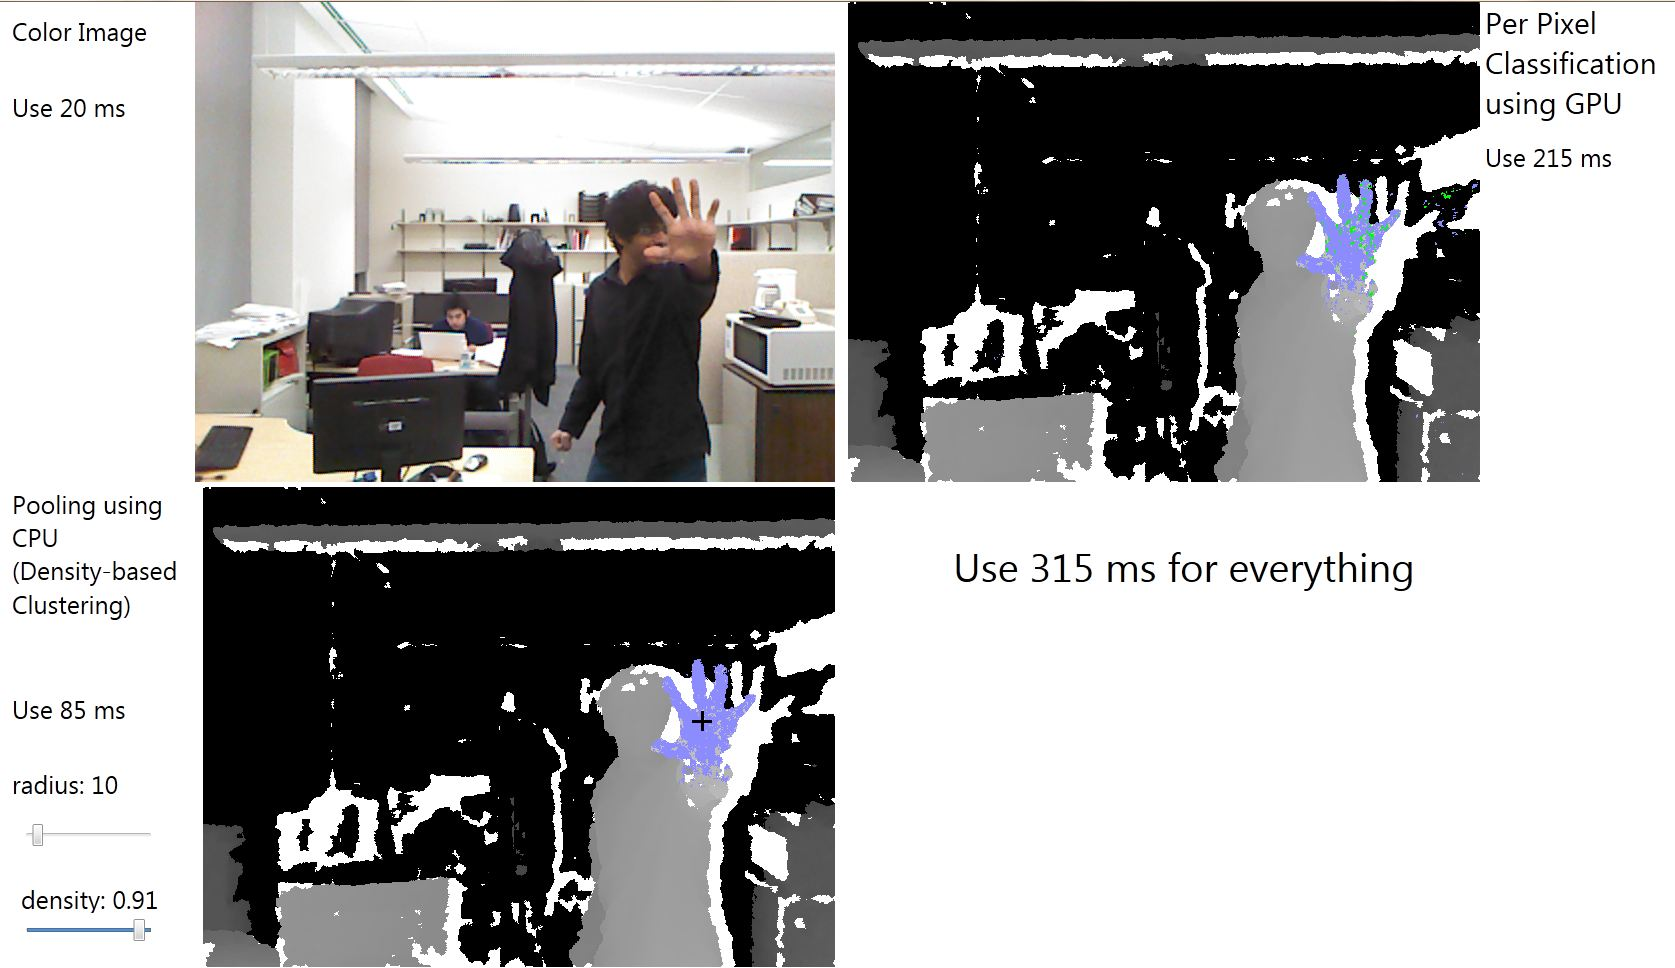
\includegraphics[width=0.5\textwidth]{fig/System.jpg}
		\cutcaption
	\caption{A snap shot of the actual system. Note the prediction is longer than it is used in a demo machine.}
\label{fig: system}
\end{figure}

We built a demo application that maps two gestures onto mouse state. The location of the hand in the XY plane determined the XY location of the mouse; moving the hand to and from the camera moved the mouse wheel up and down; and closing and opening the hand pressed down and released the left mouse button respectively. This simple mapping enabled us to navigate many applications. We successfully demonstrated this mapping on the Google Earth application \cite{googleearth} by panning and zooming the map.
